\documentclass{cslthse-msc}
\usepackage[utf8]{inputenc}
\usepackage[english]{babel}
\usepackage{amsmath}
\usepackage{amsfonts}
\usepackage{amssymb}
\usepackage{amsthm}
\usepackage{makeidx}
\usepackage{graphicx}
\usepackage[titletoc, header, page]{appendix}
\usepackage{hyperref}
\usepackage{parskip}
\usepackage[nopar]{lipsum}

% to higlight with a black rectangle when a overfull hbox occurs to make it easy to spot
\overfullrule=2cm
%\geometry{showframe}
%\author{
	David Norrestam \\
	{\normalsize \href{mailto:davidnorrestam@gmail.com}{\texttt{davidnorrestam@gmail.com}}}
	\and
	Philip Burenstam Linder \\
    {\normalsize \href{mailto:philip.burenstam.linder@gmail.com}{\texttt{philip.burenstam.linder@gmail.com}}}
}

\title{Hybrid app-development using an existing web application}
%\subtitle{A feasibility study}
\company{Lund University}

%\date{\today}
\date{Month Day, 2015}

\supervisors{Flavius Gruian, \href{mailto:Flavius.Gruian@cs.lth.se}{\texttt{Flavius.gruian@cs.lth.se}}}{Albin Willman, \href{mailto:albin.svensson@trialbee.com}{\texttt{albin.svensson@trialbee.com}}}
%\supervisor{John Deer, \href{mailto:jdeer@company.com}{\texttt{jdeer@company.com}}}
\examiner{Flavius Gruian, \href{mailto:flavius.gruian@cs.lth.se}{\texttt{flavius.gruian@cs.lth.se}}}


\acknowledgements{
We wish to offer our thanks to Trialbee for giving us the idea for this investigation and our supervisor Albin Willman who guided us and helped us develop the web application.

We would also like to take this oppurtunity to thank our examiner, Flavius Gruian at the Department of Computer Science, for all the advices and feedback he has provided throughout the process of writing this thesis.

\theabstract{
Mobile applications are today an important way for companies to reach their customers. Developing a mobile application could require a lot of resources, especially if the application is to be made from scratch. However, an alternative for a company with an existing web application, is making use of the logic in the existing web application, to create a hybrid mobile application.

In this thesis, two different approaches to developing an Android application were evaluated. The application to be developed consisted of classes for communication with native Android functions, and an encapsulated (existing) web application, making use of the functions provided by the aforementioned classes to extend its functionality. In one of the approaches, Android Framework was used for developing the hybrid application, and in the other approach, PhoneGap framework was used.

For evaluation, we recorded the development effort required in each of the two approaches, for a quantitative comparison, and also examined the structure of the developed applications, for a qualitative comparison. Development effort was estimated by measuring logical lines of code (LLoC) of the resulting application. 

The results show that a lower development effort is required when developing using PhoneGap framework, than in the Android framework. However, we noticed that developing using Android framework provides more control over the application life cycle, and can thus be a preferable option when a more advanced application needs to be developed.
}

\keywords{android, hybrid, phonegap, mobile application, web application}

%% Only used to display font sizes
\makeatletter
\newcommand\thefontsize[1]{{#1 \f@size pt\par}}
\makeatother
%%%%%%%%%%



\begin{document}
\makefrontmatter
\chapter{Introduction}
% Add text here that motivates this thesis, perhaps a quick intro 
\section{Background}
\subsection{A brief explanation of Android, hybrid applications and PhoneGap}

Android is operating system used on a wide range of devices, such as a mobile device or tv device. Coding android applications is done in the programming language Java. Code for android can be written in the official Android development environment, Android studio, but other development environment is also available. 

Android software development kit (SDK) provides the programmer with a number of tools. Such as a debugger, library, device emulator, and documentation.  

A hybrid application is a native application which is partially written with web technologies. I.e HTML5, CSS and JavaScript. The part of the application written with web technologies runs within a browsers engine in a so called WebView. A web application running in a browser does not have access to a device native functions such as the bluetooth. However a website running within a WebView can through interaction with the application's native code access a device native functions.

PhoneGap is a framework for developing mobile applications. The code is written with web technologies, the code is compiled to different platform, such as Android or IOs, specific code. The resulting application is a hybrid application. An example of a mobile application built in PhoneGap is wikipedia's mobile application.  

\section{Problem formulation}

The aim of this project is to evaluate two different development methods for encapsulating an existing web application in an Android mobile application, in order to give the web application access to the mobile's native functions. An example of such a native function would be accessing the camera of a mobile phone. It is important that the logic on the web application can be written in a general way (non-platform dependant) adapting to the device accessing the web application. This way, the method used to encapsulate the web application is easy to replace, with minimum effect on the logic of the web application. 

As the first development method, the mobile application will be built natively (in Java for android). As the second method, the mobile development framework PhoneGap will be used. The methods will be evaluated and compared from a developers perspective, with the preconditions defined section \ref{section-preconditions}

\subsection{Preconditions}\label{section-preconditions}
The study is done from a company's perspective and is based on the following prerequisites:
\begin{itemize}
\item There are only a few developers, three or less
\item There is already an existing web-application that is to be used by the mobile-application
\item The company has a need and/or desire to extend the functionality of it's web-application with native functions
\item The company's developer or developers has no prior knowledge of mobile application development
\end{itemize}

When examining the methods, the focus has been restrained to the following developing aspects
\begin{itemize}
\item Modularisation in a way so that its easy to add functionality
\item The web application should be loosely coupled with native code
\item Maintainability (easy to update in case of API change)
\end{itemize}
\section{Contribution statement}
Throughout this work we have been working together all the time. When writing code we often been pair programming and if not we have reviewed each others code afterwards. Researching has also been done together. It is therefore impossible to point to whom has done what in this thesis since all our work has been done together. 

%Om du har utför examensarbetet tillsammans med en annan student ska det i rapporten tydligt framgå vem av er som har gjort vad, både i fråga om arbetet och rapporten.

\section{Terminology}
\begin{description}
  \item[Mobile application] \hfill \\
    Refers to the application being developed, excluding code loaded from remote        websites.
  \item[Web application] \hfill \\
    If nothing else is specified it refers to the client-side of the web application.
  \item[Development methods] \hfill \\
    Refers (in the context of this paper) to the methods of mobile application          development being evaluated, i.e. using the development framework PhoneGap or       writing native Android code.
  \item[Native function] \hfill \\
     A hardware function which a device has. For example mobile with a camera and GPS have native functions when writing mobile software or applications to get access to the camera or it's GPS.
\end{description}

\chapter{Approach} \label{ch:approach}
The first section Research protocol~\ref{sec:research-protocol} describes the how the investigation of the problem formulation has been performed. The following section, Measuring Lines of Code~\ref{sec:measuring-lines-of-code}, states how the software metric logical lines of code has been used as a measurement of the result. The last section, Layer communication~\ref{sec:layer-communication}, explains how the relationship between the mobile and web application layer were evaluated. 


\section{Investigation protocol} \label{sec:investigation-protocol}
To carry out the investigation proposed in the problem formulation a practical approach has been used. To evaluate and compare the two different frameworks, a mobile application described in~\ref{subsec:the-mobile-application} was developed using each framework. The mobile application needs an existing web application and therefore a simple web application described in~\ref{subsec:the-web-application} was developed first of all. The web application was developed in the framework Ruby on Rails.

We report our experiences as developers of the web application and the mobile application in both methods. After the mobile applications were developed the architectures were visualized in UML diagrams and the different classes were described. The UML diagrams show the methods of the classes but hides the attributes of the classes for the sake of better clarity. 

\subsection{The web application} \label{subsec:the-web-application}
The front-end of the used web application consist of a single page and was developed for the web browser Google Chrome. The page displays a form with a text field, a "take photo" button, an "upload photo" button, a "location button" and a "submit button", see figure~\ref{fig:webappfront}. When the upload photo or take photo or location button is pressed the web application uses the Google Chrome’s built in ability to take or upload a photo,	 or get the location.

\begin{figure}[h!]
	\centering
    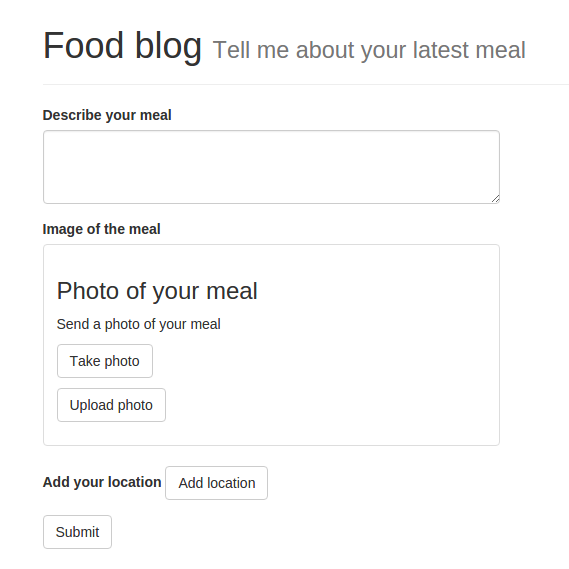
\includegraphics[width=120mm,natwidth=800,natheight=600]{./img/webAppFrontPage.png}
    \caption{The web app front page displayed in Google Chrome}
    \label{fig:webappfront}
\end{figure}

\subsection{The mobile application} \label{subsec:the-mobile-application}
The mobile application consists of two parts, the web application described above, and the mobile application encapsulating the web application. The mobile application must encapsulate the web application and display the web application the same way as it is displayed in a browser. The mobile application must use the mobile’s native functions to provide the web application with images and the mobiles location. The mobile application has no knowledge of the back-end of the web application, it merely communicates with the client-side of the web application (except for when requesting the front-end from the server).

The text field in the web application has no connection to the mobile application layer. 

For taking or uploading an image in the form, the mobile application must use an existing image from the image gallery or take a picture using the mobile camera. The photo must be passed back to the web application in Base64 format. 

The location must be obtained using the mobile’s GPS. 

When the user interacts with the mobile application, the interaction must be directly with the web application encapsulated within the mobile application. 

In the project the following equipment tools and programs were used for developing and testing:
\begin{itemize}
\item Version 21 of the Android SDK, when developing using the Android application framework
\item Apache Cordova CLI version 4.0, when developing using the PhoneGap framework
\item Android Studio, as the IDE when developing using the Android application framework
\item A regular text editor, for creating and editing JavaScript and HTML-files
\item A Nexus 5 mobile with the Android version 5.1.1, for testing the mobile applications
\item Google Chrome browser version 44.0.2403.157, for testing the web application
\end{itemize}

\section{Layer communication} \label{sec:layer-communication}
A prerequisite is that the mobile application and web application layer has a master and slave relationship. To describe this communication a flow diagram of the web layer sending a request for native data and the mobile application layer responding with data is constructed. The flow diagram acts as a suggestion in how developer friendly the communication is combined with our personal developing experiences.

\section{Measuring lines of code}\label{sec:measuring-lines-of-code}
The resulting mobile applications are measured using the software metric logical lines of code (LLoC). To count logical lines of code Project Code Meter~\cite{project-code-meter2015} has been used. Project Code Meter bases its calculation of LLoC on the Cocomo-II model~\cite{cocomo-ii-model}, and ignores the following lines of code:

\begin{itemize}
\item Auto-generated code lines
\item Header files
\item Ineffective code statements
\item Pragma compiler directives
\item Labels
\item Switch cases are not statements by themselves (so empty "case")
\item Several statements on the same physical line are counted as several LLOC
\end{itemize}

The mobile application was written in two different programming languages, Java and JavaScript. To compare the measurement result of logical lines of code the conversion table described by Galorath and Evans~\cite[p.~163]{galorath2006} was used. JavaScript and Java are both third generation languages and therefore the conversion is roughly 1 to 1. 

The logical lines of code in the web application layer were also measured in both developing methods. The resulting lines in the mobile and web application layer were added together to give a total result. 
%\chapter{Evaluation}	\label{ch:evaluation}
The evaluation is divided into four sections, first a section describing the web application developed, section~\ref{sec:web-application}, followed by one section for each framework used to develop the mobile application, sections~\ref{sec:native-android} and \ref{sec:phonegap}. Last in this chapter, is a section presenting the development effort of each mobile application, section~\ref{sec:development-effort}.

\section{Web Application}\label{sec:web-application}
The front-end of the developed web application can be found online at \url{https://github.com/DavidNorrestam/PolluxWebPhoneGap} and \url{https://github.com/DavidNorrestam/PolluxWebNative}
or in text form in appendix~\ref{app:web-app-source-code-android} and~\ref{app:web-app-source-code-phonegap}, compatible with the mobile application developed using the Android framework and the PhoneGap Framework respectively.
To simplify the process of making the web application compatible with web browsers as well as the mobile application, the architecture follows the Adapter pattern \cite[p.~317]{martin2003}. The structure of the web application can be seen in figure \ref{fig:webuml}. Items within the red dotted box belong to the structure when the Android framework was used for developing the mobile application. Items within the blue dotted box belong to the structure when the PhoneGap framework was used for developing the mobile application.

\begin{figure}[h!]
	\centering
    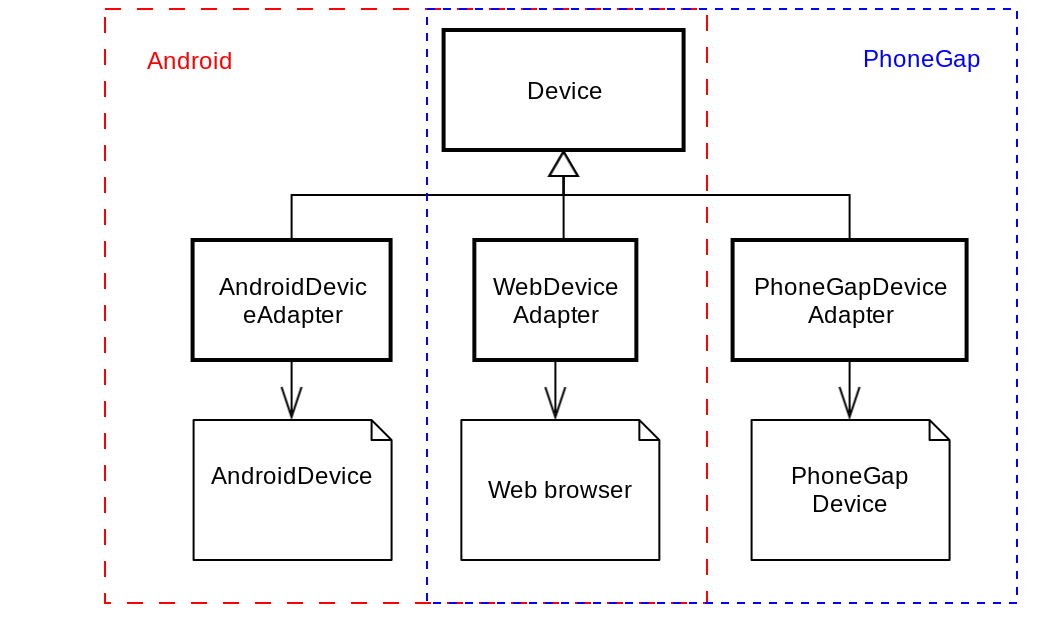
\includegraphics[width=90mm,natwidth=600,natheight=450]{./img/webuml.png}
    \caption{Structure of the web application}
	\label{fig:webuml}
\end{figure}

\section{Native android} \label{sec:native-android}
The mobile application developed in the Android framework can be found on Github at \url{https://github.com/DavidNorrestam/PolluxMobileNative}. An overview of the application structure and functionality follows in section~\ref{subsec:mobile-application-structure-native}. After this, in section~\ref{subsec:function-flow-native}, a practical example is used to describe the flow of function calls when a native function is requested by the web application layer.


\subsection{Mobile Application structure} \label{subsec:mobile-application-structure-native}
The UI of the Android application consist of a single WebView \ref{subsubsec:webview} (used to load the web application). A UML-diagram representing the logic of the Android application can be seen in figure ~\ref{fig:nativeuml}. The contained classes are summarized below, with a short explanation followed by code examples.

\begin{figure}
	\centering
    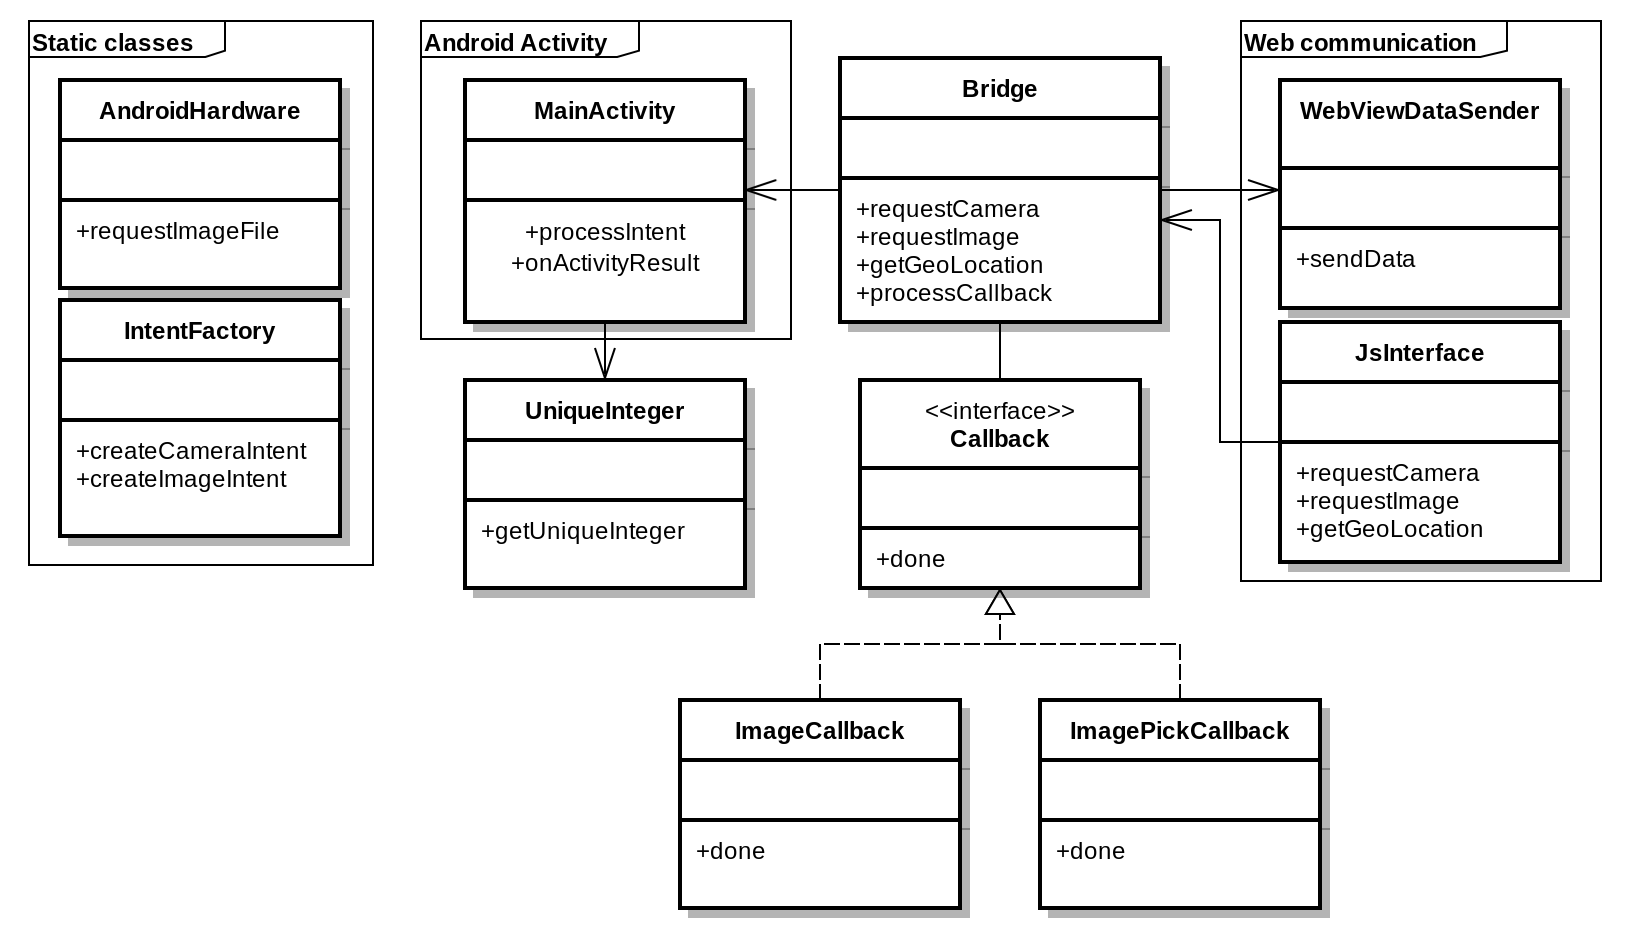
\includegraphics[width=150mm,natwidth=1000,natheight=750]{./img/polluxuml.png}
    \caption{Structure of the android application}
    \label{fig:nativeuml}
\end{figure}

\subsubsection{MainActivity} 
MainActivity is the main activity~\ref{subsubsec:activity} of the Android application. It contains logic for handling the application's activity lifecycle, and is in charge of starting any activities needed to provide the Web Application with data from native functions, such as the device camera. Activities are started by a call to the processIntent function. It takes an Intent \ref{subsubsec:intent} and a Callback (see section below) as arguments. The callback is provided a unique id, and is stored in a map. The Intent is started with the use of the startActivityForResult function provided by the Android SDK \ref{subsec:android-application-framework}, and is assigned a request id equal to the id of the Callback. 
\\\\
	
\emph{Ex. Starting an Activity for result}
\begin{lstlisting}
// Request a unique integer to use as id
int requestCode = uniqueInteger.getUniqueInteger();

// Store the Callback in a map with the unique integer as key	
callbacks.put(requestCode, callback);
   
// Start the Activity defined in the Intent, 
// assigning the unique integer as request code
startActivityForResult(intent, requestCode);
\end{lstlisting}
	
\subsubsection{IntentFactory} 
IntenFactory provides Intents \ref{subsubsec:intent} for native functions such as capturing an image or picking an image from the gallery.
	\\\\
	\emph{Ex. getting Intent from IntentFactory}
	
	\begin{lstlisting}
// In Bridge:
Intent imageIntent = IntentFactory.createCameraIntent(context);
		
// In IntentFactory:
public static Intent createCameraIntent(Context context) {
	// Create the intent for capturing an image
	Intent takePictureIntent = 
		new Intent(MediaStore.ACTION_IMAGE_CAPTURE);
	
	// Ensure that there's a camera activity to handle the intent
	if (takePictureIntent
		.resolveActivity(context.getPackageManager()) != null) {
		// Create the File where the photo should go
		File photoFile = AndroidHardware.requestImageFile();
		takePictureIntent.putExtra(MediaStore.EXTRA_OUTPUT,
		Uri.fromFile(photoFile));
	}
	return takePictureIntent;
}
\end{lstlisting}
	
\subsubsection{AndroidHardware}
AndroidHardware contains static methods, performing a single well-defined hardware related task. This design is chosen to make the application logic independent of the code in AndroidHardware. The code example below shows the function called to request a file for storing an image.
	\\\\
	\emph{Code example extracted from AndroidHardware:}
\begin{lstlisting}
public static File requestImageFile() {
 String fileName = "tempPhoto";
 File storageDir = 
   Environment.getExternalStoragePublicDirectory(
     Environment.DIRECTORY_PICTURES
     );
 File photoFile = null;
 try {
   photoFile = File.createTempFile(fileName, ".jpg", storageDir);
 } catch (IOException e) {
   e.printStackTrace();
 }
 return photoFile;
}
\end{lstlisting}
	
\subsubsection{Bridge} 
Bridge serves as a bridge between the mobile and web application layer. When the web application requests data from a native function, Bridge receives the request from JsInterface~\ref{subsubsec:jsinterface}, creates the corresponding Intent and Callback, and forwards them to MainActivity, see Ex. 1 below. Bridge also receives the result from the native function call, which it forwards to WebViewDataSender, see Ex. 2 below.
\\\\
\emph{Ex. 1 Processing a request for an image from the gallery}
\begin{lstlisting}
// Create a new intent
Intent imageIntent = IntentFactory.createImageIntent(context);

// Create callback for the intent
Callback imagePickCallback = new ImagePickCallback(this, context, callback);

// Send intent to mainActivity for processing
mActivity.processIntent(imageIntent, imagePickCallback);
\end{lstlisting}

\emph{Ex. 2 Forwarding data returned from native function}
\begin{lstlisting}
public void processCallback(String callback, String argument) {
        webViewDataSender.sendData(callback, argument);
}
\end{lstlisting}
	
\subsubsection{WebViewDataSender}
WebViewDataSender is in charge of all communication with the WebView and its encapsulated web application. Upon application start, it loads the web application and injects the JavaScriptInterface. The class also contains logic for executing JavaScript functions in the web application, used to return results from native function calls.
\\\\
\emph{Ex. sendData - used by bridge to send back results to the web application}
\begin{lstlisting}
public void sendData(final String javascriptFunction, final String arg) {
        Log.d(TAG, "sendData");
        webView.post(new Runnable() {
            	@Override
            	public void run() {
        		webView.loadUrl("javascript:" + javascriptFunction + "('" + arg + "')");
    		}
	});
}
\end{lstlisting}
	
\subsubsection{JsInterface} \label{subsubsec:jsinterface}
JsInterface is exposed to the web application as a JavaScriptInterface and acts as a receiver for function calls from the web application. If the web application requires data from a native function, the JavaScript in the web application can call upon the proper method in JsInterface, which in turn forwards the requests to Bridge.
\\\\
\emph{Ex. Two java functions exposed to the web application by JsInterface}
\begin{lstlisting}
    //Request an image from the device camera
    @JavascriptInterface
    public void requestCamera(String callback) {
        Log.d(TAG, "requestImage");
        bridge.requestCamera(callback);
    }

    // Request an image from the device storage
    @JavascriptInterface
    public void requestImage(String callback) {
        Log.d(TAG, "requestImage");
        bridge.requestImage(callback);
    }
\end{lstlisting}

	
\subsubsection{Callback} 
Callback is an interface, specifying a single public method. Classes implementing callback contain code specifying how to send results from a requested native function call back to the web application. More specifically, the code defines which JavaScript function to return the data to, and how the data is to be returned. In our solution, there are two classes implementing Callback:
	\begin{description}
		\item[ImageCallback] is used when the web application requests an image from the camera
		
		\item[ImagePickCallback] is used when the web application requests an image from the gallery
	\end{description}
		
\subsubsection{UniqueInteger} 
UniqueInteger contains a single public function getUniqueInteger, which is guaranteed to return a unique integer on each call. This is used by MainActivity when assigning a request id to an Intent and storing the corresponding Callback.

\subsection{Function flow} \label{subsec:function-flow-native}
A more detailed view of the program flow when the web application requests an image can be seen in figure ~\ref{fig:nativeflow}, further explained below.
\begin{figure}[h!]
	\centering
    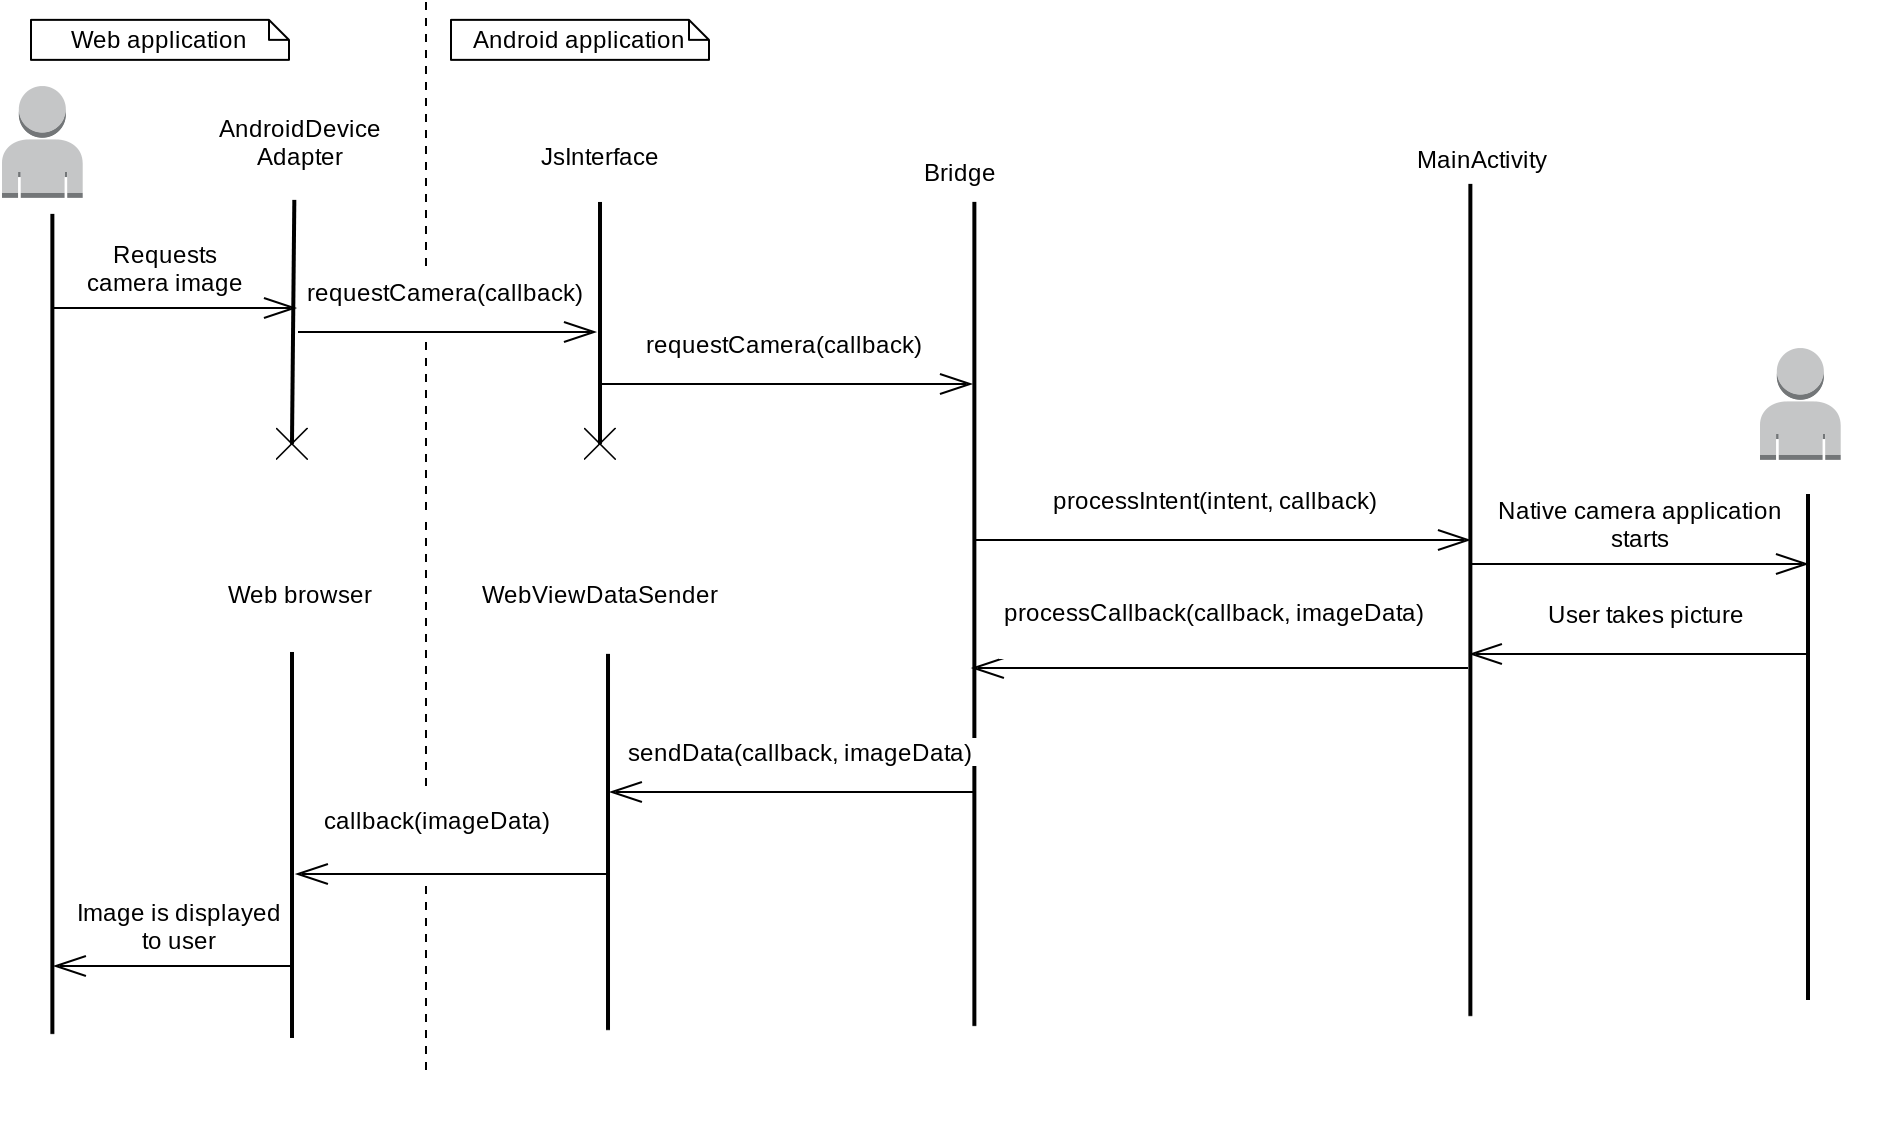
\includegraphics[width=150mm,natwidth=1000,natheight=750]{./img/androidfunctionflow.png}
    \caption{Function flowchart, single call from web application \label{fig:nativeflow}}
\end{figure}
\begin{enumerate}
	\item User action invokes a request for an image from the mobile camera.
	\item Current device adapter (see figure \ref{fig:webuml}) calls requestCamera on JsInterface, with the function name of the preferred callback function as argument.
	\item JsInterface forwards the function call to Bridge.
	\item Bridge creates the corresponding Intent and Callback, and calls processIntent on MainActivity with Intent and Callback as arguments.
	\item MainActivity gets a unique id from UniqueInteger, stores the callback in a hashmap with the id as key, and starts the intent with the id as requestcode (camera application starts).
	\item When user finishes taking a picture, the result is sent to MainActivity through onActivityResult.
	\item MainActivity finds the Callback with the same id as the processed Intent, and forwards the callback and resulting image data to Bridge through processCallback.
	\item Bridge executes the callback which in turn calls sendData on WebViewDataSender, with the image data and callback name as arguments.
	\item WebViewDataSender executes the JavaScript callback function in the WebView.
	\item The captured image is displayed to the user in the WebView.
\end{enumerate}

\section{PhoneGap}\label{sec:phonegap}
The mobile application developed in the PhoneGap framework can be found on Github at \url{https://github.com/DavidNorrestam/PolluxMobilePhoneGap}. An overview of the application structure and functionality follows in section~\ref{subsec:application-structure-phonegap}. After this, in section~\ref{subsec:function-flow-phonegap}, a practical example is used to describe the flow of function calls when a native function is requested by the web application layer.


\subsection{Mobile application structure} \label{subsec:application-structure-phonegap}
The Android application developed using PhoneGap is a hybrid application~\ref{sec:terminology}, and is thus run within a WebView on Android. The user interface of the developed application is a HTML document containing a single IFrame~\ref{sec:iframe}, which is used to load the web application front-end. To be able to embed the web application front-end the X-Frame-Options response header were removed. The logic developed for the Android application is written in JavaScript, which is loaded in the WebView. A UML-diagram representing the logic of the Android application can be seen in figure~\ref{fig:phonegapuml}, with the classes summarized below.
\begin{figure}[h!]
	\centering
    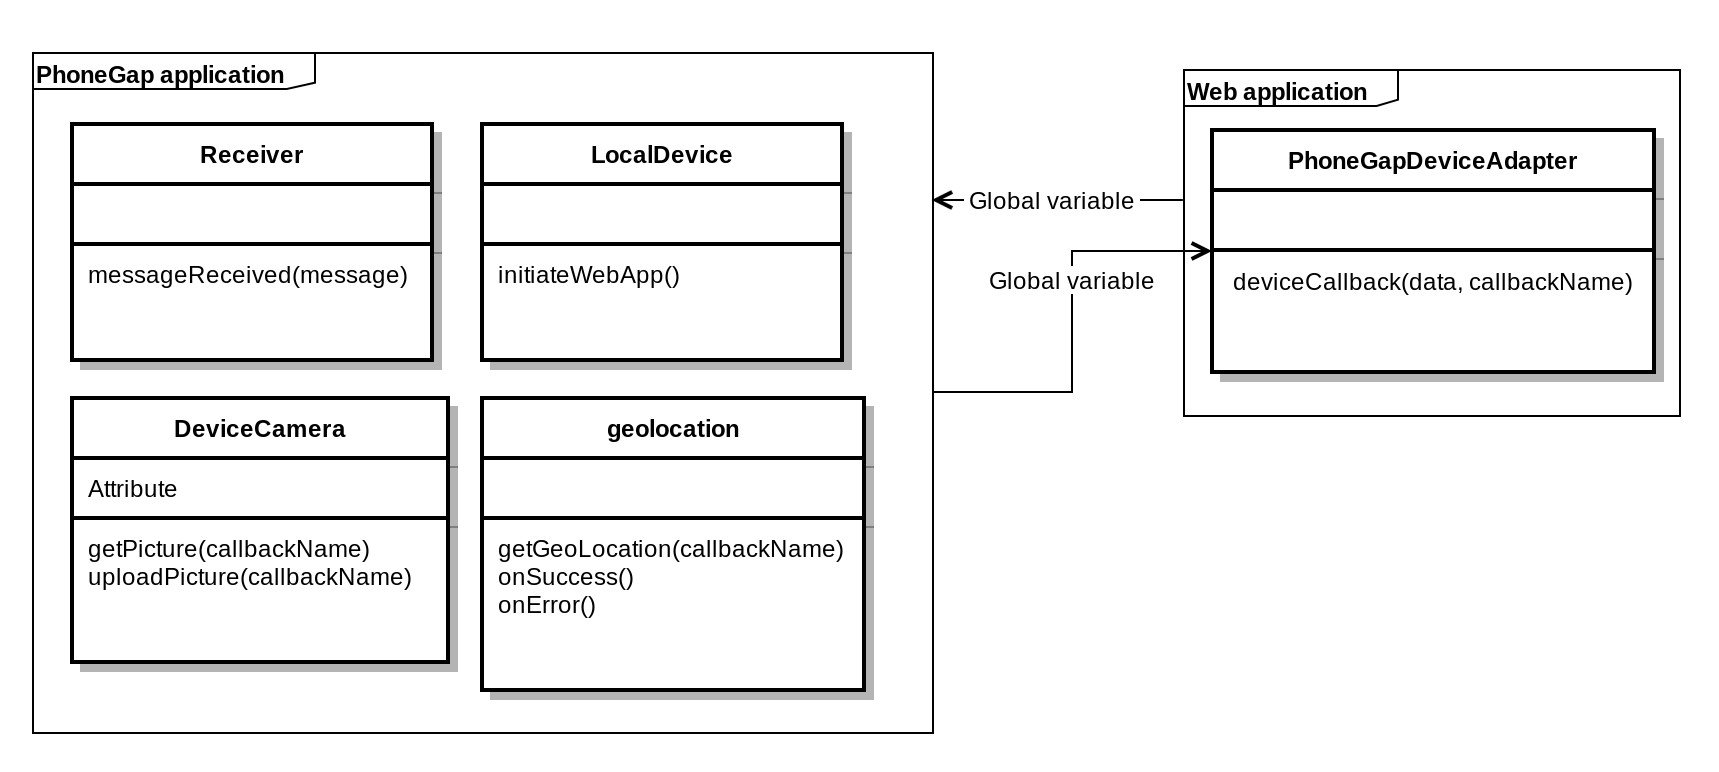
\includegraphics[width=150mm,natwidth=1000,natheight=750]{./img/phonegapuml.png}
    \caption{Structure of the PhoneGap application}
    \label{fig:phonegapuml}
\end{figure}

\subsubsection{Receiver}
Receiver listens to messages posted by the web application layer. A message contains a request for data from a native feature.
\label{fig:phonegapflow}
\subsubsection{LocalDevice}
LocalDevice contains a single method initiateWebApp, which is used to load the web application in an IFrame and initialize device, see figure~\ref{fig:webuml}, in the web application to the correct adapter.

\subsubsection{DeviceCamera}
DeviceCamera contains logic for invoking and receiving results from the device camera. Communication with the device camera is handled by functions provided by the PhoneGap framework. Its functions are called by Receiver upon requests from the web application layer.

\subsubsection{geolocation}
Geolocation contains logic for accessing the mobile's geolocation (GPS-position). Its functions are called by Receiver upon requests from the web application.

\subsection{Function flow}\label{subsec:function-flow-phonegap}
A more detailed view of the program flow when the web application requests an image can be seen in figure~\ref{fig:phonegapflow}, further explained below.
\begin{figure}[h!]
	\centering
    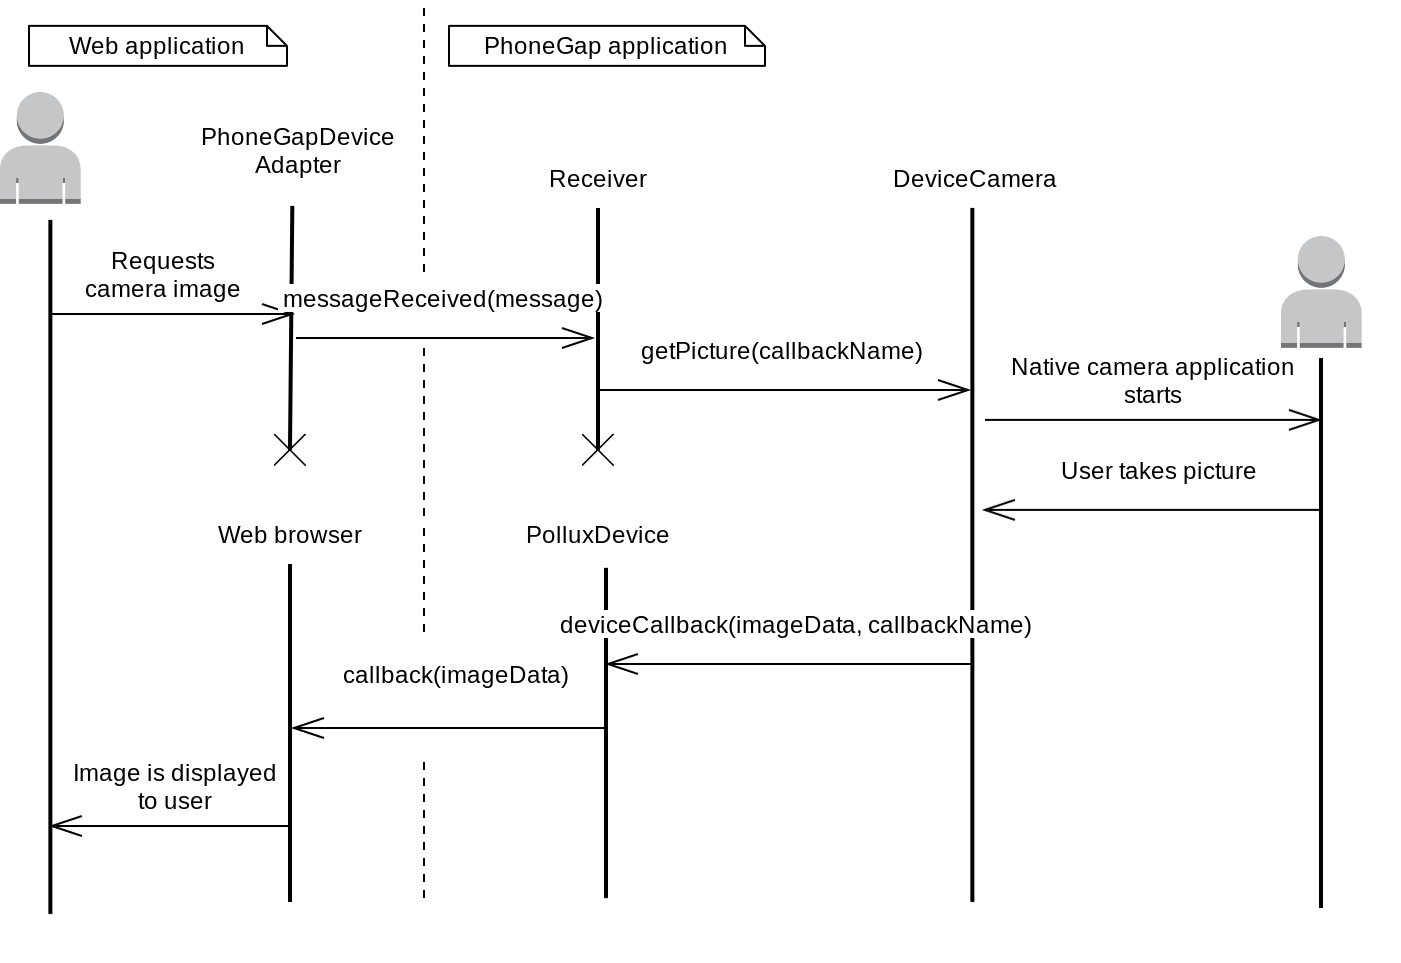
\includegraphics[width=120mm,natwidth=800,natheight=600]{./img/phonegapfunctionflow.png}
    \caption{Function flowchart, single call in web application \label{fig:phonegapflow}}
\end{figure}
\begin{enumerate}
	\item User action invokes a request for an image from the mobile camera. 
	\item Current device adapter (PhoneGapDeviceAdapter) forwards the request to the mobile application using postMessage.
	\item The message gets processed by the PhoneGap receiver which forwards the call to DeviceCamera via the getPicture function.
	\item DeviceCamera starts the camera application.
	\item When user is finished taking a picture, the result is returned to DeviceCamera.
	\item DeviceCamera returns the result to the IFrame by invoking DeviceCallback on the exposed JavaScript object, in the mobile application known as PolluxDevice.
	\item DeviceCallback calls the JavaScript callback function specified in its argument.
	\item The captured image is displayed to the user in the WebView.
\end{enumerate}


\section{Development effort}\label{sec:development-effort}
The development effort was measured using lines of code as described in section~\ref{sec:measuring-lines-of-code}. A summary of the results can be seen in the table below.

\begin{tabular}{ | l | c | r | }
    \hline
    \multicolumn{3}{|c|}{Lines of code - mobile application} \\
    \hline
	Metric & Using Android SDK &  Using PhoneGap \\
	\hline
	Files & 10 & 3\\
	LLoC & 200 & 86\\	
	\hline
	\multicolumn{3}{c}{\emph{Result of code evaluation using ProjectCodeMeter}}
\end{tabular}

\begin{tabular}{ | l | c | r | }
    \hline
    \multicolumn{3}{|c|}{Lines of code - web application} \\
    \hline
	Metric & Using Android SDK & Using PhoneGap \\
	\hline
	Files & 2 & 2 \\
	LLoC & 173 & 175 \\	
	\hline
	\multicolumn{3}{c}{\emph{Result of code evaluation using ProjectCodeMeter}}
\end{tabular}


%\chapter{Discussion} \label{ch:discussion}
The problem formulation in section~\ref{sec:problem-formulation} can be summarized to:
What are the differences in code structure and development effort for two different development methods for encapsulating an existing web application in a mobile application to utilize native functions?

Our results show that developing such a mobile application in the PhoneGap framework requires less development effort than in the Android framework. A reason for this might be that calls to native functions are handled on a higher abstraction level. Another reason is that 10 classes were used in the Android framework compared to an eqvuivalent to 4 classes in the PhoneGap framework.

The structure that we suggested in the Android framework is modular, separating creation of a request for a native function, handling of the data passed back from the request and communication with the web application layer. The PhoneGap framework also separates the communication with the web application layer, but a request for a native function and handling of the data passed back is located in the same file. 

The mobile application developed in the PhoneGap framework has fewer steps from receiving a request from the web application layer to pass the data back, see flowchart~\ref{fig:nativeflow} and~\ref{fig:phonegapflow}. This suggests that the application developed in the PhoneGap framework has a less complex structure then the application developed in Android framework.

The PhoneGap framework has a higher abstraction level of calls to native functions. That allows for fewer logical lines of code, but there is a downside. The downside is that one has less freedom in terms of customizing the behavior. The loss of freedom makes no difference for a simple mobile application such the one developed, but as Kohan and Montanez points out for a more complex application it might be a problem, see section~\ref{subsec:phonegap}. 

In the Android framework there is a closer relation to the Android System/Hardware, however this comes with a requirement of boilerplate code. That is one of the reasons that the mobile application that was developed in the Android framework had more than double the logical lines of code. This closer relation means that the developer can have a better control over the application lifecycle. The closer relation also means that basic knowledge of Android is needed. If the developer has no prior knowledge of Android this means a starting cost. 

Encapsulating the web application front-end in the PhoneGap framework was made at the cost of a security flaw. The web application front-end was encapsulated by use of an IFrame. To be able to use an IFrame the web applications X-Frame-Options response header was removed which makes it possible to use the web application for ClickJacking, see section~\ref{sec:iframe}. 

There are other ways of encapsulating the front-end of a web application in the PhoneGap framework than by using an IFrame. Another way would be to use a plugin that is available in the PhoneGap API called inAppBrowser. By using inAppBrowser a web page can be loaded into the mobile application and the mobile application layer can execute the web page’s JavaScript functions. If the web page would like to send a request to the mobile application layer the mobile application layer can listen to such requests by the use of polling.  This could be an alternative to using an IFrame that would not expose the web application to be used for ClickJacking. 

To compare the development effort the software metric logical lines of code were used. Logical lines of code were chosen since it is easy to understand, measurable between two programming languages and simple to calculate. Other ways of measuring lines of code or other software metrics could have been used to measure development effort or other properties. To measure more properties and also measure development effort in other ways would have provided a more nuanced result and a fuller picture. For example Halsted's approach, described in section~\ref{sec:lines-of-code}, could have been used to measure the development effort. Another property that could have been measured would have been cyclomatic complexity. Cyclomatic complexity measures the number of linearly independent paths through a program’s source code. 

The result of this study is drawn from one small and simple project. This makes it hard to draw any conclusions about using the two development methods for medium and large projects. It raises the question whether developing in the PhoneGap framework in bigger projects or using more advanced features would still score lower in development effort. One interesting question would be whether the proposed structure in the development methods provide a good bone structure for more complex projects? Or would the structure crumble? The measurement and proposed structure is based on this single project. To get a more reliable result it would be interesting to collect data from a number of projects where a mobile application, encapsulating an existing web application, has been developed in both development methods.

The structure we proposed in the web application, to be able to run both in a web browser and in a mobile application, makes use of the adapter pattern. This makes it easy to further extend web applications functionality. If a new function has no connection to native functionality, such as an animation, the function can be implemented as if the mobile application did not exist. When new functionality is needed which includes native functionality, such as getting information from the accelerometer, then the web application need at least three functions. The first function is needed to make the request to the mobile application and a second function is needed which determines the functionality on a browser. Finally a function which handles the data which is passed back from the request. 

%\chapter{Conclusions} \label{ch:conclusions}
The aim of this thesis has been to investigate the process of developing an Android application which encapsulates, and extends an existing web application with native functionality. The investigation was performed by developing said Android application using two different frameworks, the Android framework and the PhoneGap framework, and evaluating the advantages and drawbacks of each framework.

The development approaches were evaluated qualitatively by recording the development effort required, and quantitatively by examining the structure of the developed application. The development effort was estimated by measuring the number of logical lines of code (LLoC) of the developed application.

The results show that it is preferable to use PhoneGap when low development effort is important. However, when security is important, the application structure proposed in this paper is not recommended, due to the risk of allowing the web application to be embedded in an iframe.
When using the PhoneGap framework, development is only done using web technologies. Therefore, it is also preferable to use the PhoneGap framework if the developer has more experience working with web technologies than working with Java. 

However, the Android framework is to prefer if it is important to have more control over the application lifecycle, a closer relation to the Android system or hardware, and not be limited by a library. The Android framework is also to prefer if the security risk that is introduced with the use of an inline frame in the PhoneGap framework is not acceptable.

Although our investigation has reached its aims, the choice of scope of the investigation introduces limitations to the study. 
First, because of the time limit and lack of resources, the study was only performed for the Android platform. 
Second, only a small project was investigated, which makes it hard to draw conclusions for medium and large size projects. 
Third, the result is based on the development of a single mobile application. To be able to draw conclusions in the general case, it would be necessary to investigate the development of multiple applications of different size and nature. 
Fourth, only very simple native functionality was used, therefore it is hard to draw conclusions about the development effort when more advanced functionality is needed.

One interesting conclusion we draw from our investigation is that the development effort is significantly lower when the PhoneGap framework is used. This contradicts Kohan and Montanez, who estimated that the development effort for a small to medium sized project for an Android mobile application would be the same in the PhoneGap and Android framework. However, their estimation is based on that the mobile application is built from scratch.
\begin{thebibliography}{9}

\bibitem{galorath2006}
Daniel D. Galorath and Michael W. Evans, \emph{Software Sizing, Estimation, and Risk Management}, Auerbach Publications, Taylor and Francis Group, 2006.
  
\bibitem{fenton2015}
Norman Fenton, Queen Mary University of London, UK, James Bieman, Colorado State University, Fort Collins, USA, \emph{Software Metrics: A Rigorous and Practical Approach}, CRC Press, Taylor and Francis Group, 3rd edition, 2015
  
\bibitem{kohan2015}
Bernard Kohan and Joseph Montanez,
\emph{Native vs Hybrid/PhoneGap App Development Comparison},
  \url{http://www.comentum.com/phonegap-vs-native-app-development.html},
  Comentum, San Diego,
  January 26, 2015
  
\bibitem{harris2010}
	Online survey from Harris Interactive on behalf of EffectiveUI,
	United States,
September 30 - October 4, 2010

\bibitem{pcmlloc2015}
	Project Code Meter - Logical Lines of Code,
	\url{http://www.projectcodemeter.com/cost_estimation/help/GL_lloc.htm},
September 8, 2015

\bibitem{michaels2013}
	Michaels, Ross \& Cole, ltd,
	\emph{Native mobile apps: The wrong choice for business?}
	\url{http://www.mrc-productivity.com/research/whitepapers/NativeAppsWrongChoice.pdf},
	Lombard, IL,
January 2013

% info taken from http://www.gartner.com/newsroom/id/2996817
\bibitem{gartner2015}
	Gartner, Inc
	\emph{Market Share: Devices, All Countries, 4Q14 Update},
	\url{ http://www.gartner.com/document/2985017},
	Stamford, Connecticut, USA,
March 2015

%http://mashable.com/2011/05/12/ice-cream-sandwich/#GIRObYC0nqkO
\bibitem{dell2011}
	Jolie O'Dell, 
	\emph{Androids Unite: How Ice Cream Sandwich Will End the OS Schism},
	\url{ http://mashable.com/2011/05/12/ice-cream-sandwich/#GIRObYC0nqkO},
	May 2011

%https://en.wikipedia.org/wiki/Software_framework#cite_note-1 first source in the article
\bibitem{riehle2000}
	Dirk Riehle, 
	\emph{Framework Design: A Role Modeling Approach},
	Swiss Federal Institute of Technology,
	2000
	
\bibitem{eclipse2012}
	Eclipse Open Source Developer Report, 
	\url{http://www.slideshare.net/IanSkerrett/eclipse-survey-2012-report-final},
	2012
	
\bibitem{mondal2013}
	Shruti Mukherjee , Ishani Mondal, 
	\emph{Future Practicability of Android Application Development with New Android Libraries and Frameworks },
	Narula Institute of Technology, 
	Institute of Engineering and Management,
	November 2013 
	
\bibitem{androiddevelopers2015}
	Android Developers,
	\url{http://developer.android.com},
	September 2015

\bibitem{titanium15}
	Appcelerator Titanium,
	\url{https://www.appcelerator.com/product/},
	September 2015

\bibitem{stay-away1-titanium15}
	Sam Moffatt,
	\emph{A few months with Titanium Appcelerator},
	\url{http://pasamio.com/2011/07/02/a-few-months-with-titanium-appcelerator/},
	July 2011

\bibitem{stay-away2-titanium15}
	Andre Adallera,
\emph{Why you should stay away from Appcelerator’s Titanium},
\url{https://usingimho.wordpress.com/2011/06/14/why-you-should-stay-away-from-appcelerators-titanium/},
	June 2011

\bibitem{tech-republic-jquery-mobile-compatible14}
Jacob Orshalick,
\emph{Create cross-platform apps with PhoneGap and jQuery Mobile},
\url{http://www.techrepublic.com/blog/software-engineer/create-cross-platform-apps-with-phonegap-and-jquery-mobile/},
	Tech Republic,
	January 2014
	
\bibitem{project-code-meter2015}
	Project Code Meter, 
	\url{http://www.projectcodemeter.com/cost_estimation/help/GL_lloc.htm},
	September 2015

\bibitem{cocomo-ii-model}
	Cocomo-II model,
	\url{http://sunset.usc.edu/research/COCOMOII/Docs/modelman.pdf},
	October 2015

\bibitem{jquery-mobile15}
	JQuery Mobile homepage,
	\url{https://jquerymobile.com/},
	September 2015

\bibitem{martin2003}
	Robert Cecil Martin,
	\emph{Agile software development, principles patterns and practices},
	Pearson Education Inc,
	2003	

\bibitem{law2010}
	Eric Law,
	\emph{Combating ClickJacking With X-Frame-Options},
	\url{https://developer.mozilla.org/en-US/docs/Web/HTTP/X-Frame-Options},
	Telerik,
	March 2010
\end{thebibliography}
\end{document}